%% Beispiel-Präsentation mit LaTeX Beamer im KIT-Design
%% https://sdq.kastel.kit.edu/wiki/Dokumentvorlagen
\documentclass{sdqbeamer}

%% ----------------------------------------------------------------
%% PACKAGES
%% ----------------------------------------------------------------
\usepackage[utf8]{inputenc}
\usepackage[T1]{fontenc}
\usepackage{listings}
\usepackage{xcolor}
\usepackage{booktabs}
\usepackage{tikz}
\usetikzlibrary{positioning, arrows.meta, shapes, calc, fit}
\usepackage{amsmath}
\usepackage{amssymb}

%% ----------------------------------------------------------------
%% CODE STYLING
%% ----------------------------------------------------------------
\definecolor{codegreen}{rgb}{0,0.6,0}
\definecolor{codegray}{rgb}{0.5,0.5,0.5}
\definecolor{codepurple}{rgb}{0.58,0,0.82}
\definecolor{backcolour}{rgb}{0.95,0.95,0.92}

\lstdefinestyle{pythonstyle}{
    backgroundcolor=\color{backcolour},
    commentstyle=\color{codegreen},
    keywordstyle=\color{magenta},
    numberstyle=\tiny\color{codegray},
    stringstyle=\color{codepurple},
    basicstyle=\ttfamily\scriptsize,
    breakatwhitespace=false,
    breaklines=true,
    captionpos=b,
    keepspaces=true,
    numbers=left,
    numbersep=5pt,
    showspaces=false,
    showstringspaces=false,
    showtabs=false,
    tabsize=2,
    language=Python
}
\lstset{style=pythonstyle}

\usepackage[citestyle=numeric,bibstyle=numeric,hyperref,backend=biber]{biblatex}
\addbibresource{presentation.bib}
\bibhang1em

%% ----------------------------------------------------------------
%% METADATA & SETUP
%% ----------------------------------------------------------------

%% Gruppenlogo (Optional)
\grouplogo{kl.png}

%% Gruppenname
\groupname{Praxis der Forschung - SotA Presentatio}

%% Titel & Autor
\title[Double Machine Learning for Spatio-Temporal Conflict Data]{State-of-the-Art Presentation: DML for Spatio-Temporal Conflict Data}
\subtitle{State-of-the-Are Presentation | Scientific Computing Center (SCC) -- Methods for Big Data}
\author[Niklas Bitzer]{Niklas Bitzer}
\date{26.11.2025}

%% ----------------------------------------------------------------
%% DOCUMENT START
%% ----------------------------------------------------------------
\begin{document}

%% 1. TITLE PAGE
% Using the standard template option 'title reen horizontal'
% If you have a background image, add: picture=path/to/image
\begin{frame}[title green horizontal, kitlogo=white]
	\titlepage
\end{frame}


%% 2. TABLE OF CONTENTS
% Using the template option to color the TOC
\begin{frame}[tableofcontents=green]{Contents}
	\tableofcontents
\end{frame}

%% ----------------------------------------------------------------
%% CONTENT SECTIONS
%% ----------------------------------------------------------------

\section{Introduction}

\begin{frame}{Introduction}{Conflict Data}
    \begin{columns}[t]
        \column{0.48\textwidth}
        \begin{greenblock}{Recent Data Revolution}
            \textbf{Characteristics}
            \begin{itemize}
                \item High-dimensional
                \item Fine-grained
                \item Spatio-temporal
            \end{itemize}
            \textbf{Sources}
            \begin{itemize}
                \item Conflict Event Databases (UCDP GED \cite{sundberg_introducing_2013}; ACLED \cite{raleigh_introducing_2010})
                \item Remote Sensing: Climate variables; Satellite imagery \cite{racek_conflict_2024}
                \item Structural Embeddings: Economic/Social indicators \cite{rod_review_2024}
            \end{itemize}
            \vspace*{\fill}
        \end{greenblock}

        \column{0.48\textwidth}
		\vspace*{-4cm}
        \begin{royalblueblock}{Example from \textcite{racek_capturing_2025}}
            \begin{itemize}
                \item PRIO-GRID covering Africa
                \item $0.5^\circ \times 0.5^\circ$ lattice grid structure ($55 \times 55$ km² at the equator)
                \item 10,640 grid cells
                \item Monthly data from 2000 to 2020 (252 months)
            \end{itemize}
            \vspace*{\fill}
        \end{royalblueblock}
            \centering
            \begin{figure}
                \includegraphics[width=0.65\linewidth, height=\textheight, keepaspectratio]{img2.png}
            \end{figure}

    \end{columns}
\end{frame}

\begin{frame}{Introduction}{Application of Conflict Research}
    \begin{columns}[t]
        \column{0.55\textwidth}
        \textbf{Goals:}
        \begin{itemize}
            \item Predict conflict (where and when)
            \item Prevent conflict
            \item Guide post-conflict recovery
            \item \textbf{Explain underlying causal mechanisms}
            \item \textbf{Evaluate causal impact}
            \vspace{0.3em}
        \end{itemize}
        \textbf{Stakeholders:}
        \begin{itemize}
            \item Policymakers
            \item Humanitarian Organizations
            \item Early Warning Systems
        \end{itemize}

        \column{0.42\textwidth}
        \begin{royalblueblock}{Key Areas}
            \textbf{Specific Interventions:}
            \begin{itemize}
                \item Foreign aid allocation \cite{kuzmanovic_causal_2024}
                \item Military actions \cite{papadogeorgou_causal_2022}
            \end{itemize}
            \textbf{External Shocks:}
            \begin{itemize}
                \item Economic shocks \cite{miguel_economic_2004}
                \item Climate events
            \end{itemize}
        \end{royalblueblock}
    \end{columns}
\end{frame}

\begin{frame}{Introduction}{Fundamental Challenges}
    \begin{columns}[t]
        \column{0.31\textwidth}
        \begin{redblock}{1. Interpretability}
            \begin{itemize}
                \item Policymakers take no action without trust \cite{rudin_stop_2019}
                \item Forecasting models identify \textbf{correlates, not causes} \cite{cederman_predicting_2017}
                \item Prediction $\rightarrow$ Explanation is the key challenge
            \end{itemize}
        \end{redblock}

        \column{0.31\textwidth}
        \begin{redblock}{2. Dimensionality}
            \textbf{High-Dimensional Setting \cite{hegre_introducing_2020}}
            \begin{itemize}
                \item Covariates $\gg$ Observations
                \item Hundreds of confounders
                \item Traditional methods fail
                \item \textbf{Need}: Regularization (Lasso, RF)
                \item \textbf{But}: Regularization $\rightarrow$ Bias \cite{belloni_high-dimensional_2014}
            \end{itemize}
        \end{redblock}

        \column{0.31\textwidth}
        \begin{redblock}{3. Conflict Diffusion}
            \textbf{Spatial Dependencies}
            \begin{itemize}
                \item Spillover effects across grid cells
                \item SUTVA violations (interference) \cite{papadogeorgou_causal_2022}
            \end{itemize}
            \vspace{0.3em}
            \textbf{Temporal Dependencies}
            \begin{itemize}
                \item Conflict persistence
                \item Carryover effects \cite{racek_capturing_2025}
            \end{itemize}
        \end{redblock}
    \end{columns}
\end{frame}

\section{From Forecasting to Causal Inference}

\begin{frame}{From Forecasting to Causal Inference}{SotA in Forecasting}
    \begin{lightgraybox}
        Forecasting has moved beyond small-scale country-specific designs to fine-grained event data \cite{croicu_forecasting_2025}.
    \end{lightgraybox}

    \vspace{1em}

    \begin{columns}[t]
        \column{0.48\textwidth}
        \begin{itemize}
            \item \textbf{Methodological Approaches \cite{hegre_202324_2025}:}
            \begin{itemize}
                \item Non-parametric Ensembles: Random Forests, XGBoost
                \item Deep Learning: LSTMs, Transformers (e.g. Temporal Fusion Transformers)
                \item LLMs based on news corpora
            \end{itemize}
            \item VIEWS competition \cite{hegre_202324_2025} represents the benchmark
            \item \textbf{Performance:} High predictive accuracy for static risk assessment
        \end{itemize}

        \column{0.48\textwidth}
        \begin{redblock}{Limitations \cite{cederman_predicting_2017, racek_capturing_2025}}
            \begin{itemize}
                \item Lack interpretability (\textbf{Black Box Models})
                \item Limited capabilities at predicting conflict dynamics (e.g., onsets, escalations)
                \item Spatial dependence often treated as nuisance
                \item Spatial/temporal lags used as simple controls
            \end{itemize}
        \end{redblock}
    \end{columns}
\end{frame}

\begin{frame}{From Forecasting to Causal Inference}{The Missing Causal Understanding}
    % Added [t] here to fix the alignment issue you mentioned
    \begin{columns}[t]
        \column{0.48\textwidth}
        \begin{blueblock}{Forecasting Goal}
            \textbf{Maximize Predictive Accuracy}
            \begin{itemize}
                \item Objective: $\min \mathbb{E}[(Y - \hat{Y})^2]$
                \item Metrics: AUROC, Brier score
                \item Question: ``What happens next?''
            \end{itemize}
        \end{blueblock}

        \column{0.48\textwidth}
        \begin{blueblock}{Causal Goal}
            \textbf{Identify Treatment Effects}
            \begin{itemize}
                \item Structural Parameter: $\theta_0$ or $\tau(x)$
                \item Valid Inference: $\sqrt{n}(\hat{\theta} - \theta_0) \to \mathcal{N}(0, \Sigma)$
                \item Question: ``What if we intervene?''
            \end{itemize}
        \end{blueblock}
    \end{columns}

    \vspace{1em}

    \begin{redblock}{Good Prediction is not Enough}
        \begin{itemize}
            \item Distinct epistemological goals \cite{shmueli_explain_2010}
            \item Correlation $\neq$ Causation
            \item ``Theory-free prediction does little to guide intervention without knowledge about the drivers of conflict'' \cite[p.23]{cederman_predicting_2017}
            \item Policy decisions require \textbf{counterfactual reasoning} \cite{feuerriegel_causal_2024}.
        \end{itemize}
    \end{redblock}
\end{frame}

\begin{frame}{From Forecasting to Causal Inference}{Causal Machine Learning}
    \begin{columns}
        \column{0.95\textwidth}
        \begin{redblock}{The Fundamental Problem of Causal Inference \cite{holland_statistics_1986}}
            The inability to observe both treated and untreated potential outcomes for the same unit simultaneously.
        \end{redblock}
    \end{columns}

    \vspace{1em}

    % Added [t] here to align the text on the right with the list on the left
    \begin{columns}[t]
        \column{0.48\textwidth}
        \textbf{The Approach \cite{athey_machine_2019}:}
        \begin{itemize}
            \item Combines flexible estimation of ML with principles from causal inference
            \item Builds on potential outcomes framework
            \item Enables effect estimation for high-dimensional covariates \& complex non-linear relations
        \end{itemize}

        \column{0.48\textwidth}
        \textbf{Heterogeneity:} \\
        New methodological approaches focus on \textbf{Heterogeneous Treatment Effects (HTE)} by estimating the \textbf{Conditional Average Treatment Effect (CATE)} \cite{kunzel_metalearners_2019}.

        \vspace{0.8em}

        \textbf{Taxonomy:}
        \begin{itemize}
            \item Tree-based methods (Causal Forests \cite{wager_estimation_2017})
            \item Meta-learners (T/S/X-Learner) \cite{kunzel_metalearners_2019}
            \item Orthogonalization (DML \cite{chernozhukov_doubledebiased_2018})
        \end{itemize}
    \end{columns}
\end{frame}

\section{Saptio-Temporal Causal Inference}

\begin{frame}{Spatio-Temporal Causal Inference}{SUTVA Violation}
    \begin{columns}[T]
        \column{0.65\textwidth}

    \textbf{The Assumption:} Stable Unit Treatment Value Assumption (SUTVA)
    \begin{equation*}
        Y_i(w_1, \dots, w_N) = Y_i(w_i) \quad \text{(Independence of units)}
    \end{equation*}

            \textbf{Fails for Conflict Data \cite{racek_capturing_2025}}
            \begin{itemize}
                \item \textbf{Spillover (Spatial Interference)}
				% Treatment in cell A affects outcome in cell B
                \item \textbf{Carryover (Temporal Persistence)}
				% Effects of an intervention persist even after treatment has ended
            \end{itemize}

            \vspace{0.5em}
            \begin{greenblock}{Explicit Modelling}
			\begin{itemize}
			\item Network/Dependecy Graph \cite{leung_treatment_2020}
			\item Geometry/Ring Methods \cite{pollmann_causal_2023}
			\item Nonparametric Smoothing \cite{racek_capturing_2025}
			\item Stochastic Point Processes \cite{papadogeorgou_causal_2022}
							\end{itemize}
            \end{greenblock}

        \column{0.35\textwidth}
		\vspace*{-4cm}
            \centering
            \begin{figure}
                \includegraphics[width=\linewidth, height=0.9\textheight, keepaspectratio]{img1.png}
            \end{figure}
    \end{columns}
\end{frame}

\begin{frame}{Spatio-Temporal Causal Inference}{Spatial Confounding}
    \begin{columns}[T]
        \column{0.55\textwidth}
		\textbf{Interference vs. Confounding}
		\begin{itemize}
			\item Interference: Outcomes spill over
			\item Confounding: Clusters in space
		\end{itemize}
\vspace*{0.5em}
        \textbf{The Assumption:} Unconfoundedness (Ignorability)
        \begin{redblock}{Fails for Spatial Data}
            \textbf{Spatial Confounding:} Unmeasured variables $U$ with spatial structure affect both treatment and outcome.
            \begin{itemize}
			\item Conflict drivers are not randomly distributed
                \item \textbf{Latent Variables ($U_i$):} Governance, terrain, ethnic tensions, culture
                \item $\Rightarrow$ spurious treatment-outcome association
            \end{itemize}
        \end{redblock}
        \column{0.41\textwidth}
            \centering
        \begin{tikzpicture}[
            node distance=2cm,
            box/.style={rectangle, draw, minimum width=2cm, minimum height=1.5cm, font=\small},
            latent/.style={circle, draw, dashed, minimum size=2cm, font=\small},
            arrow/.style={->, >=stealth, thick}
        ]
            \node[box] (W) {$W$};
            \node[box, right=of W] (Y) {$Y$};
            \node[box, above=0.8cm of W] (X) {$X$};
            \node[latent, above=0.8cm of Y] (U) {$U$};

            \draw[arrow] (W) -- (Y);
            \draw[arrow] (X) -- (W);
            \draw[arrow] (X) -- (Y);
            \draw[arrow, color=kit-red100] (U) -- (W);
            \draw[arrow, color=kit-red100] (U) -- (Y);
        \end{tikzpicture}
		\vspace{1.25em}
            \begin{greenblock}{Mitigation Strategies}
                \begin{itemize}
                    \item Spatial Fixed Effects (if static)
                    \item Spatial Basis Functions
                    \item Distance-adjusted matching
                \end{itemize}
            \end{greenblock}
    \end{columns}
\end{frame}

\begin{frame}{Spatio-Temporal Causal Inference}{Other Challenges}
    \begin{columns}[T]
        \column{0.48\textwidth}

        \begin{redblock}{i.i.d. Assumption Violated}
            \textbf{Standard ML \& Inference assume:}
            \begin{equation*}
                (Y_i, W_i, X_i) \overset{\text{i.i.d.}}{\sim} P
            \end{equation*}

            \textbf{Spatio-temporal data:}
            \begin{equation*}
                \text{Cov}(Y_{it}, Y_{js}) \neq 0
            \end{equation*}

            % {\small for units $i, j$ nearby or times $t, s$ close}
        \end{redblock}

        \column{0.48\textwidth}

        \begin{royalblueblock}{Dynamic Treatment Effects}
            Effects unfold over time:
            \begin{equation*}
                Y_{it} = \sum_{\ell=0}^{L} \theta_\ell \, W_{i,t-\ell} + g_0(X_{it}) + \varepsilon_{it}
            \end{equation*}

            % {\small $\theta_\ell$ = causal effect at lag $\ell$}
        \end{royalblueblock}

        \vspace{0.3em}

        \begin{redblock}{Challenges}
        \begin{itemize}
            \item \textbf{Carryover Effets:} $W_{t-1} \to Y_t$
            \item \textbf{Feedback Loops:} $Y_{t-1} \to W_t$
            \item \textbf{Time-varying confounding}
        \end{itemize}
		\end{redblock}

        % \vspace{0.3em}

        % {\small \textit{E.g., aid allocated because of past conflict}}

    \end{columns}
\end{frame}

\section{Double Machine Learning}

\begin{frame}{Double Machine Learning}{The Basics}
    \begin{columns}[T]
        \begin{column}{0.48\textwidth}
           \textbf{The Problem:}
           \begin{itemize}
               \item Naive ML estimation of $\eta$ introduces regularization bias.
               \item $\Rightarrow$ slower than $\sqrt{N}$ convergence for $\hat{\theta}$.
           \end{itemize}

           \vspace{0.5cm}
    \begin{greenblock}{Neyman Orthogonality}
        Score $\psi$ is Neyman orthogonal if the moment condition is insensitive to local perturbations in the nuisance parameter $\eta$:
        $$ \partial_{\eta} E[\psi(W; \theta_0, \eta_0)][\eta - \eta_0] = 0 $$
        \textbf{Result:} We can plug in noisy estimates $\hat{\eta}$ without creating first-order bias.
    \end{greenblock}
        \end{column}

        \begin{column}{0.48\textwidth}
            \begin{center}
                \textbf{The DML Algorithm:}
            \end{center}
            \begin{enumerate}
                \item \textbf{Split} data into $K$ folds (Cross-Fitting).
                \item \textbf{Predict} nuisances using ML:
                \[ \hat{Y} = \hat{g}(X), \quad \hat{D} = \hat{m}(X) \]
                \item \textbf{Residualize}:
                \[ \tilde{Y} = Y - \hat{Y}, \quad \tilde{D} = D - \hat{D} \]
                \item \textbf{Regress} residuals to find causal effect:
                \[ \tilde{Y} = \theta \tilde{D} + \epsilon \]
            \end{enumerate}
        \end{column}
    \end{columns}
\end{frame}

\begin{frame}{Double Machine Learning}{Cross-Fitting for Spatio-Temporal Data}
\begin{columns}{T}
	\begin{column}{0.56\textwidth}

    Standard DML assumes independent observations (i.i.d.)
	Our data is:
    \begin{itemize}
        \item \textbf{Spatially Correlated:} Conflict spills over borders.
        \item \textbf{Temporally Dependent:} History matters.
    \end{itemize}

    \vspace{0.3cm}
	\begin{greenblock}{Solutions}
    \begin{itemize}
        \item \textbf{Block Cross-Fitting:}
        Split by Time Blocks or Spatial Clusters to preserve dependence structure
        \item \textbf{Multiway Clustering:}
        Standard errors must clustered by Grid ID and Time ID % \cite{chiang_multiway_2022}.
    \end{itemize}
	\end{greenblock}
	\end{column}
	\begin{column}{0.40\textwidth}

    \centering
    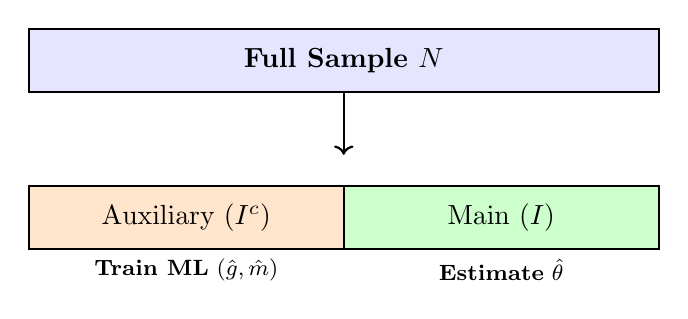
\begin{tikzpicture}[xscale=2, yscale=0.8]
        % Fold 1
        \draw[fill=blue!10, thick] (0,1) rectangle (4,2);
        \node at (2,1.5) {\textbf{Full Sample $N$}};

        % Arrow
        \draw[->, thick] (2,1) -- (2,0);

        % Splits
        \draw[fill=orange!20, thick] (0,-1.5) rectangle (2,-0.5);
        \node at (1,-1) {Auxiliary ($I^c$)};
        \node[below, font=\footnotesize] at (1,-1.5) {\textbf{Train ML} ($\hat{g}, \hat{m}$)};

        \draw[fill=green!20, thick] (2,-1.5) rectangle (4,-0.5);
        \node at (3,-1) {Main ($I$)};
        \node[below, font=\footnotesize] at (3,-1.5) {\textbf{Estimate} $\hat{\theta}$};

    \end{tikzpicture}
	\end{column}
	\end{columns}
\end{frame}

\begin{frame}{Double Machine Learning}{Methodologies \& Research Questions}
    \vspace{1em}
    \begin{columns}[t]
        \column{0.31\textwidth}
        \begin{blueblock}{RQ1: Drivers}
            \centering \textbf{Standard DML} \\ (PLR)
            \vspace{0.5em}
            \begin{itemize}
			\item Which explainable causes drive the spatio-temporal diffusion of armed conflict?
			\item \textbf{Challenges:} Spatial Confounding, Identifiability
            \end{itemize}
            % \vspace{0.5em}
            % \tiny Ref: \cite{chernozhukov_doubledebiased_2018}
        \end{blueblock}

        \column{0.31\textwidth}
        \begin{blueblock}{RQ2: Diffusion over Time}
            \centering \textbf{DML \& DTE} \\ (Panel Data)
            \vspace{0.5em}
            \begin{itemize}
			\item How does the treatment effect diffuse conflicts over time?
			\item \textbf{Challenges:} DTE Challenges / Dynamic Confounding
                % \item \footnotesize How do effects propagate over time? (Impulse Response)
            \end{itemize}
            % \vspace{0.5em}
            % \tiny Ref: \cite{lewis_doubledebiased_2021}
        \end{blueblock}

        \column{0.31\textwidth}
        \begin{blueblock}{RQ3: Interactions}
            \centering \textbf{DML \& HTE} \\ (CATE)
            \vspace{0.5em}
            \begin{itemize}
			\item Which covariates have an interaction effect with the treatment's diffusion?
			\item \textbf{Challenges:} High-Dimensionality, Identifiability
                % \item \footnotesize Which covariates moderate the effect?
            \end{itemize}
            % \vspace{0.5em}
            % \tiny Ref: \cite{semenova_debiased_2021}
        \end{blueblock}
    \end{columns}
\end{frame}

\begin{frame}{Double Machine Learning}{DML for Dynamic Treatment Effects (Lemis \& Syrgkanis 2021)}
    \begin{columns}[T]
        \begin{column}{0.48\textwidth}
                \textbf{Partially Linear Markovian Model}

                \vspace{0.2cm}

                Treatments over time affect:
                \begin{itemize}
                    \item Future states (through system dynamics)
                    \item Future treatments (through policy)
                    \item Future outcomes (directly + indirectly)
                \end{itemize}

                \vspace{0.2cm}

                \textbf{Goal:} Estimate effect of treatment at period $t$ on final outcome, at different time lags

                \vspace{0.2cm}

                \textbf{Key Innovation:} Sequential peeling to isolate causal effects at each lag

    % {\footnotesize Generalizes to Structural Nested Mean Models (SNMMs)}

            \vspace{0.3cm}
        \end{column}

        \begin{column}{0.48\textwidth}
            % Visual Timeline
            \begin{royalblueblock}{Dynamic DML Algorithm}
                \textbf{For each time lag}:

                \vspace{0.2cm}

                \textbf{1. Residualize outcome}
                \begin{itemize}
                    \item Use ML to predict final outcome from state
                    \item Compute outcome residuals
                \end{itemize}

                \textbf{2. Residualize treatments}
                \begin{itemize}
                    \item Use ML to predict past treatments from state
                    \item Compute treatment residuals
                \end{itemize}

                \textbf{3. Estimate effect}
                \begin{itemize}
                    \item Regress outcome residuals on treatment residuals
                    \item Account for previously estimated lags
                \end{itemize}

                \vspace{0.2cm}
            \end{royalblueblock}
			\end{column}

    \end{columns}
\end{frame}

\begin{frame}{Double Machine Learning}{DML for Heterogeneous Treatment Effects}
    \begin{columns}[T]
        \begin{column}{0.48\textwidth}
            \begin{royalblueblock}{Conditional Average Treatment Effect (CATE)}
                \textbf{CATE:} $\tau(x) = E[Y_i(1) - Y_i(0) \mid X_i = x]$

                \vspace{0.2cm}

                Treatment effect for units with characteristics $x$


                \textbf{Problem:}
				\begin{itemize}
					\item true CATE are not readily observable
					\item infinitely dimensional (only aggregated measuers)
				\end{itemize}
                \textbf{Solution:} Approximate with low-dimensional projection
            \end{royalblueblock}

            \vspace{0.2cm}

            \begin{royalblueblock}{Best Linear Predictor (BLP)}
                \textbf{Approximate:}
                \begin{equation*}
                    \tau(x) \approx \alpha + \beta_1 x_1 + \beta_2 x_2 + \cdots + \beta_p x_p
                \end{equation*}
				with $\alpha$ ATE and $\beta_j$ how $x_j$ modifis the effect
            \end{royalblueblock}
        \end{column}

\begin{column}{0.48\textwidth}
            \begin{royalblueblock}{Methodology (DML Procedure)}
                \textbf{Step 1: Nuisance Estimation (ML)}
                \begin{itemize}
                    \item Split sample (Cross-Fitting)
                    \item Predict outcome $\hat{g}(Z) = E[Y|Z]$
                    \item Predict treatment $\hat{m}(Z) = E[D|Z]$
                \end{itemize}

                \textbf{Step 2: Orthogonalization}
                Compute residuals to remove confounding:
                \begin{equation*}
                    \tilde{Y} = Y - \hat{g}(Z), \quad \tilde{D} = D - \hat{m}(Z)
                \end{equation*}

                \textbf{Step 3: Linear Projection}
                Regress outcome residuals on treatment interactions:
                \begin{equation*}
                    \tilde{Y} = \alpha \tilde{D} + \sum \beta_j (\tilde{D} \cdot x_j) + \epsilon
                \end{equation*}
            \end{royalblueblock}
        \end{column}
    \end{columns}
\end{frame}

\section{Research Gap}

%% ----------------------------------------------------------------
%% APPENDIX & BACKUP
%% ----------------------------------------------------------------
\appendix
\beginbackup

% \begin{frame}[allowframebreaks]{References}
% 	\begin{thebibliography}{99}

% 		\bibitem{racek2025capturing}
% 		Racek, D., Thurner, P. W., \& Kauermann, G. (2025). Capturing the Spatio-Temporal Diffusion Effects of Armed Conflict: A Nonparametric Smoothing Approach. \textit{Journal of the Royal Statistical Society: Series A}.

% 		\bibitem{racek2024conflict}
% 		Racek, D., Thurner, P. W., Davidson, B. I., Zhu, X., \& Kauermann, G. (2024). Conflict Prediction Using Remote Sensing Data: An Application to Syria. \textit{International Journal of Forecasting, 40}(1), 373--391.

% 		\bibitem{fritz2022role}
% 		Fritz, C., Mehrl, M., Thurner, P. W., \& Kauermann, G. (2022). The Role of Governmental Weapons Procurements in Forecasting Monthly Fatalities in Intrastate Conflicts. \textit{International Interactions, 48}(4), 778--799.

% 		\bibitem{chernozhukov2018double}
% 		Chernozhukov, V., Chetverikov, D., Demirer, M., Duflo, E., Hansen, C., Newey, W., \& Robins, J. (2018). Double/debiased machine learning for treatment and structural parameters. \textit{The Econometrics Journal, 21}(1), C1--C68.

% 		\bibitem{robinson1988root}
% 		Robinson, P. M. (1988). Root-N-consistent semi-parametric regression. \textit{Econometrica, 56}, 931--954.

% 	\end{thebibliography}
% \end{frame}

\backupend

\end{document}
